\documentclass[12pt]{article}

\usepackage{xcolor}
\usepackage{float}
\usepackage{graphicx}
\usepackage{fancyhdr}

\usepackage[utf8]{inputenc}
\usepackage{setspace}

\usepackage[dvips,letterpaper,margin=1in]{geometry}

\setlength{\parindent}{0pt}
\setlength{\headheight}{15pt} % fancyhdr wants at least 14.5pt

% Header
\pagestyle{fancy}
\lhead{MFRFS K3 Xeon-D Interface Description}
\rhead{July 28, 2020}
\renewcommand{\headrulewidth}{0.4pt}
\renewcommand{\footrulewidth}{0.4pt}

% Start document
\begin{document}

%%%%%%%%%%%%%%%%%%%% Title Page %%%%%%%%%%%%%%%%%%%%%%%%
\thispagestyle{empty}
\begin{titlepage}
\begin{center}
        \vspace*{1cm}

        \LARGE{Multi-Function Radio Frequency System (MFRFS) K3 \\
            Xeon-D Interface Description}

        \vspace{0.5cm}
        \LARGE
        % Subtitle

        \vspace{1.5cm}

        \normalsize

        John Jesus \\
        July 28, 2020

        \vfill



        \vspace{0.8cm}




\end{center}
\end{titlepage}

\tableofcontents
\newpage

%%%%%%%%%%%%%%%%% Start of Body %%%%%%%%%%%%%%%%%%%%%%%%
\section{Scope}
\subsection{Purpose}
This document is describes interfaces to the Xeon-D SoC of the XES Xpedite7674 Single Board Computer as planned for MFRFS K3.

\subsection{References}
\begin{enumerate}
    \item XPedite7674 Users Manual Revision C (Extreme Engineering Solutions, February 1, 2018) \label{ref:board_man}
    \item XIt1088 User’s Manual Revision A (Extreme Engineering Solutions, May 29, 2019) \label{ref:rtm_man}
    \item XPEDITE7674 Schematic Diagram SCH90030490 Revision C (Extreme Engineering Solutions, February 28, 2020) \label{ref:schematic}
\end{enumerate}

\section{Interfaces}

Interfaces are depicted in Figure \ref{fig:inteface}.  Details of each interface are provided in subsections below.

\begin{figure}[H]
\begin{center}
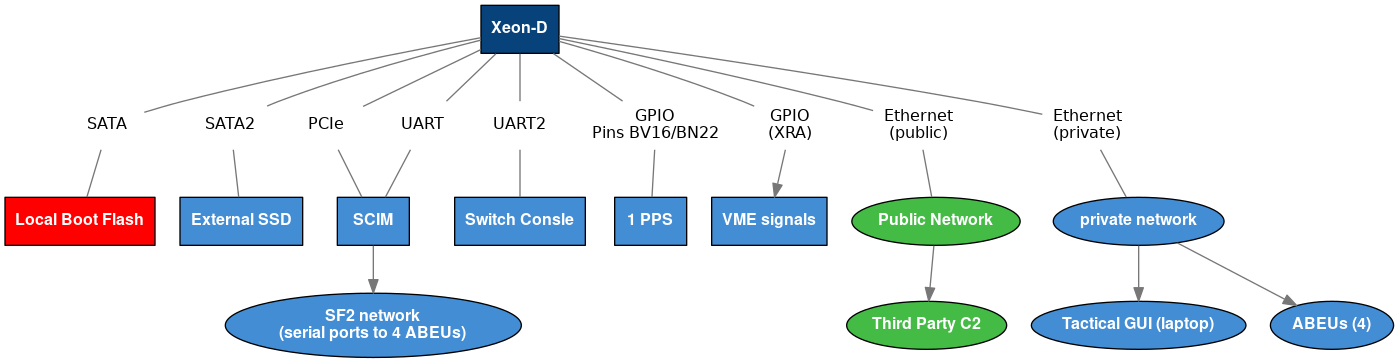
\includegraphics[width=1.0\textwidth]{img/interface}
\caption{Xeon-D Interfaces on the XPedite7674 for MFRFS K3}
\label{fig:inteface}
\end{center}
\end{figure}


% %%%%%%%%%%%%%%%%%%%%%%%%%%%%%%%%%%%%%%%%%%%%%%%
% sata (boot flash)
% %%%%%%%%%%%%%%%%%%%%%%%%%%%%%%%%%%%%%%%%%%%%%%%

\subsection{SATA (local boot flash)}
\label{section:sata}

This SATA interface is to the Linux boot image and initial ram disk.  The K3 application does not use this interface. An entry in \texttt{/etc/services.d} in the initial ram disk starts a K3 application called \texttt{CSWMain} which is a shim program that loads the K3 application from the External SSD (Section \ref{section:sata2}).


% %%%%%%%%%%%%%%%%%%%%%%%%%%%%%%%%%%%%%%%%%%%%%%%
% sata2 (external ssd)
% %%%%%%%%%%%%%%%%%%%%%%%%%%%%%%%%%%%%%%%%%%%%%%%

\subsection{SATA (External SSD)}
\label{section:sata2}


\end{document}

